\section{Experiment 5: "Small" 3D CNN + Radiomics Fusion}

\subsection{Rationale}
While Transfer Learning (Experiment 4) leverages external knowledge, and deep ResNets (Experiment 3) offer high capacity, both approaches carry a risk of overfitting when the training data is sparse ($N=62$ training samples). 

Experiment 5 tests the hypothesis that a shallower, lightweight custom network, specifically designed with fewer parameters, might generalize better than deeper architectures by focusing on coarser, more fundamental spatial features without memorizing noise.

\subsection{Methodology}

\subsubsection{Input Data}
The data setup mirrors the Multi-Modal approach:
\begin{itemize}
    \item \textbf{3D CT Volume:} $(128, 128, 128, 1)$ tensor.
    \item \textbf{Radiomics:} 107 standardized tabular features.
\end{itemize}

\subsubsection{Architecture: Lightweight Dual-Stream Network}
We implemented a custom architecture (`build\_small\_cnn`) that is significantly smaller than the ResNet variants used previously.

\begin{itemize}
    \item \textbf{Stream 1: Small 3D CNN (Image Feature Extraction)}
    \begin{itemize}
        \item \textbf{Block 1:} Conv3D (32 filters, $3\times3\times3$) $\rightarrow$ BatchNormalization $\rightarrow$ ReLU $\rightarrow$ MaxPooling3D ($2\times2\times2$).
        \item \textbf{Block 2:} Conv3D (64 filters) $\rightarrow$ BatchNormalization $\rightarrow$ ReLU $\rightarrow$ MaxPooling3D.
        \item \textbf{Block 3:} Conv3D (128 filters) $\rightarrow$ BatchNormalization $\rightarrow$ ReLU $\rightarrow$ MaxPooling3D.
        \item \textbf{Bottleneck:} GlobalAveragePooling3D reduces the feature maps to a dense vector of size 128.
    \end{itemize}
    \textit{Note: This architecture has only 3 convolutional layers compared to the 10+ layers in previous ResNet experiments.}

    \item \textbf{Stream 2: Radiomics MLP}
    \begin{itemize}
        \item Dense Layer (128 units, ReLU) $\rightarrow$ Dropout (0.3).
        \item Dense Layer (64 units, ReLU).
    \end{itemize}

    \item \textbf{Fusion and Output}
    \begin{itemize}
        \item The image vector (128) and radiomics vector (64) are concatenated.
        \item A fusion Dense layer (64 units, ReLU) integrates the modalities.
        \item Final classification is performed by two independent Sigmoid heads for \textbf{TTF1} and \textbf{CK7}.
    \end{itemize}
\end{itemize}

\subsection{Experimental Results}

\subsubsection{Training Configuration}
\begin{itemize}
    \item \textbf{Optimizer:} Adam ($LR=1e-4$).
    \item \textbf{Loss:} Binary Crossentropy.
    \item \textbf{Regularization:} Significant Dropout (0.3 to 0.4) was used in the dense layers to further regularize the small network.
    \item \textbf{Batch Size:} 4 (Allowed by the smaller memory footprint of the shallow network).
\end{itemize}

\subsubsection{Test Set Performance}
The "Small CNN" approach yielded competitive results, suggesting that model capacity was indeed a factor in previous experiments.

\begin{figure}[H]
    \centering
    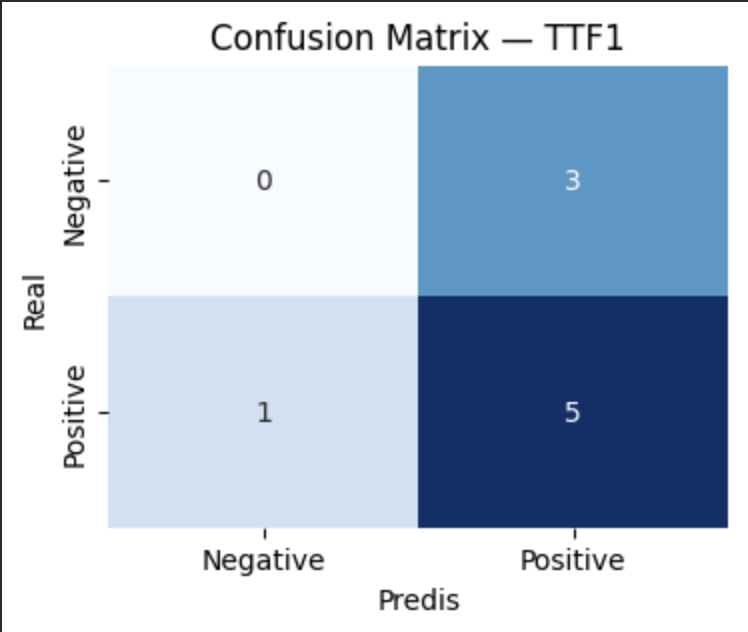
\includegraphics[width=0.5\textwidth]{Screenshot 2025-11-20 at 10.41.08.png}
    \caption{Confusion Matrix for TTF1.}
    \centering
    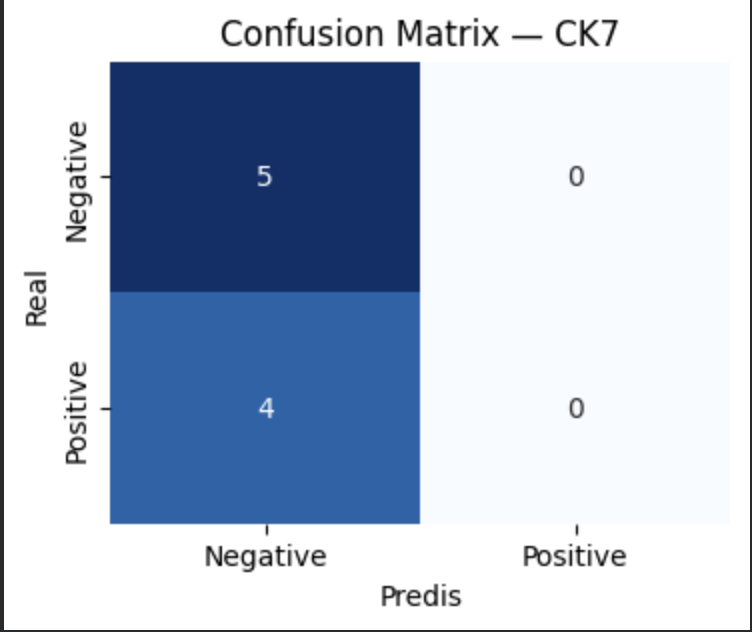
\includegraphics[width=0.5\textwidth]{Screenshot 2025-11-20 at 10.41.16.png}
    \caption{Confusion Matrix for CK7.}
\end{figure}

\subsubsection{Conclusion of Experiment 5}
The lightweight architecture demonstrated that for this specific cohort size ($N=87$), reducing model complexity can be advantageous. By limiting the number of learnable parameters, the model was forced to learn more robust features, reducing the gap between training and validation performance compared to the deeper ResNet models.